\documentclass[twoside]{book}

% Packages required by doxygen
\usepackage{fixltx2e}
\usepackage{calc}
\usepackage{doxygen}
\usepackage{graphicx}
\usepackage[utf8]{inputenc}
\usepackage{makeidx}
\usepackage{multicol}
\usepackage{multirow}
\PassOptionsToPackage{warn}{textcomp}
\usepackage{textcomp}
\usepackage[nointegrals]{wasysym}
\usepackage[table]{xcolor}

% Font selection
\usepackage[T1]{fontenc}
\usepackage{mathptmx}
\usepackage[scaled=.90]{helvet}
\usepackage{courier}
\usepackage{amssymb}
\usepackage{sectsty}
\renewcommand{\familydefault}{\sfdefault}
\allsectionsfont{%
  \fontseries{bc}\selectfont%
  \color{darkgray}%
}
\renewcommand{\DoxyLabelFont}{%
  \fontseries{bc}\selectfont%
  \color{darkgray}%
}
\newcommand{\+}{\discretionary{\mbox{\scriptsize$\hookleftarrow$}}{}{}}

% Page & text layout
\usepackage{geometry}
\geometry{%
  a4paper,%
  top=2.5cm,%
  bottom=2.5cm,%
  left=2.5cm,%
  right=2.5cm%
}
\tolerance=750
\hfuzz=15pt
\hbadness=750
\setlength{\emergencystretch}{15pt}
\setlength{\parindent}{0cm}
\setlength{\parskip}{0.2cm}
\makeatletter
\renewcommand{\paragraph}{%
  \@startsection{paragraph}{4}{0ex}{-1.0ex}{1.0ex}{%
    \normalfont\normalsize\bfseries\SS@parafont%
  }%
}
\renewcommand{\subparagraph}{%
  \@startsection{subparagraph}{5}{0ex}{-1.0ex}{1.0ex}{%
    \normalfont\normalsize\bfseries\SS@subparafont%
  }%
}
\makeatother

% Headers & footers
\usepackage{fancyhdr}
\pagestyle{fancyplain}
\fancyhead[LE]{\fancyplain{}{\bfseries\thepage}}
\fancyhead[CE]{\fancyplain{}{}}
\fancyhead[RE]{\fancyplain{}{\bfseries\leftmark}}
\fancyhead[LO]{\fancyplain{}{\bfseries\rightmark}}
\fancyhead[CO]{\fancyplain{}{}}
\fancyhead[RO]{\fancyplain{}{\bfseries\thepage}}
\fancyfoot[LE]{\fancyplain{}{}}
\fancyfoot[CE]{\fancyplain{}{}}
\fancyfoot[RE]{\fancyplain{}{\bfseries\scriptsize Generated on Fri Apr 29 2016 15\+:35\+:25 for My Project by Doxygen }}
\fancyfoot[LO]{\fancyplain{}{\bfseries\scriptsize Generated on Fri Apr 29 2016 15\+:35\+:25 for My Project by Doxygen }}
\fancyfoot[CO]{\fancyplain{}{}}
\fancyfoot[RO]{\fancyplain{}{}}
\renewcommand{\footrulewidth}{0.4pt}
\renewcommand{\chaptermark}[1]{%
  \markboth{#1}{}%
}
\renewcommand{\sectionmark}[1]{%
  \markright{\thesection\ #1}%
}

% Indices & bibliography
\usepackage{natbib}
\usepackage[titles]{tocloft}
\setcounter{tocdepth}{3}
\setcounter{secnumdepth}{5}
\makeindex

% Hyperlinks (required, but should be loaded last)
\usepackage{ifpdf}
\ifpdf
  \usepackage[pdftex,pagebackref=true]{hyperref}
\else
  \usepackage[ps2pdf,pagebackref=true]{hyperref}
\fi
\hypersetup{%
  colorlinks=true,%
  linkcolor=blue,%
  citecolor=blue,%
  unicode%
}

% Custom commands
\newcommand{\clearemptydoublepage}{%
  \newpage{\pagestyle{empty}\cleardoublepage}%
}


%===== C O N T E N T S =====

\begin{document}

% Titlepage & ToC
\hypersetup{pageanchor=false,
             bookmarks=true,
             bookmarksnumbered=true,
             pdfencoding=unicode
            }
\pagenumbering{roman}
\begin{titlepage}
\vspace*{7cm}
\begin{center}%
{\Large My Project }\\
\vspace*{1cm}
{\large Generated by Doxygen 1.8.7}\\
\vspace*{0.5cm}
{\small Fri Apr 29 2016 15:35:25}\\
\end{center}
\end{titlepage}
\clearemptydoublepage
\tableofcontents
\clearemptydoublepage
\pagenumbering{arabic}
\hypersetup{pageanchor=true}

%--- Begin generated contents ---
\chapter{Class Index}
\section{Class List}
Here are the classes, structs, unions and interfaces with brief descriptions\+:\begin{DoxyCompactList}
\item\contentsline{section}{\hyperlink{struct__Mensaje}{\+\_\+\+Mensaje} \\*Mensaje }{\pageref{struct__Mensaje}}{}
\item\contentsline{section}{\hyperlink{structAula}{Aula} \\*\hyperlink{structAula}{Aula} }{\pageref{structAula}}{}
\end{DoxyCompactList}

\chapter{File Index}
\section{File List}
Here is a list of all documented files with brief descriptions\+:\begin{DoxyCompactList}
\item\contentsline{section}{\hyperlink{ej4a_8c}{ej4a.\+c} \\*El ejercicio 4a de la Practica 1 S\+O\+P\+E\+R }{\pageref{ej4a_8c}}{}
\item\contentsline{section}{\hyperlink{ej4b_8c}{ej4b.\+c} \\*El ejercicio 4b de la Practica 1 S\+O\+P\+E\+R }{\pageref{ej4b_8c}}{}
\item\contentsline{section}{\hyperlink{ej5a_8c}{ej5a.\+c} \\*El ejercicio 5a de la Practica 1 S\+O\+P\+E\+R }{\pageref{ej5a_8c}}{}
\item\contentsline{section}{\hyperlink{ej5b_8c}{ej5b.\+c} \\*El ejercicio 5b de la Practica 1 S\+O\+P\+E\+R }{\pageref{ej5b_8c}}{}
\item\contentsline{section}{\hyperlink{ej8a_8c}{ej8a.\+c} \\*El ejercicio 8a de la Practica 1 S\+O\+P\+E\+R }{\pageref{ej8a_8c}}{}
\item\contentsline{section}{\hyperlink{ej8b_8c}{ej8b.\+c} \\*El ejercicio 8b de la Practica 1 S\+O\+P\+E\+R }{\pageref{ej8b_8c}}{}
\item\contentsline{section}{\hyperlink{ejercicio6_8c}{ejercicio6.\+c} \\*El ejercicio 6 de la Practica 1 S\+O\+P\+E\+R }{\pageref{ejercicio6_8c}}{}
\item\contentsline{section}{\hyperlink{ejercicio9_8c}{ejercicio9.\+c} \\*El ejercicio 9 de la Practica 1 S\+O\+P\+E\+R }{\pageref{ejercicio9_8c}}{}
\end{DoxyCompactList}

\chapter{Class Documentation}
\hypertarget{struct__Mensaje}{\section{\+\_\+\+Mensaje Struct Reference}
\label{struct__Mensaje}\index{\+\_\+\+Mensaje@{\+\_\+\+Mensaje}}
}


Mensaje.  




{\ttfamily \#include $<$semaforos.\+h$>$}

\subsection*{Public Attributes}
\begin{DoxyCompactItemize}
\item 
long \hyperlink{struct__Mensaje_a216a370cde3eae04df6a81fea5bef338}{id}
\item 
char \hyperlink{struct__Mensaje_a89a493b8d3c3e803d637fbdcfbd1bdab}{aviso} \mbox{[}4 $\ast$1024+1\mbox{]}
\item 
int \hyperlink{struct__Mensaje_a4980e5d47c0feeda94157d1fdbac9fe6}{pid}
\item 
int \hyperlink{struct__Mensaje_a47abc67c07fe0d5eaf709a4a9ad59129}{aula}
\end{DoxyCompactItemize}


\subsection{Detailed Description}
Mensaje. 

Esta estructura define un mensaje. 

\subsection{Member Data Documentation}
\hypertarget{struct__Mensaje_a47abc67c07fe0d5eaf709a4a9ad59129}{\index{\+\_\+\+Mensaje@{\+\_\+\+Mensaje}!aula@{aula}}
\index{aula@{aula}!\+\_\+\+Mensaje@{\+\_\+\+Mensaje}}
\subsubsection[{aula}]{\setlength{\rightskip}{0pt plus 5cm}int \+\_\+\+Mensaje\+::aula}}\label{struct__Mensaje_a47abc67c07fe0d5eaf709a4a9ad59129}
\hyperlink{structAula}{Aula} donde esta asignado el alumno \hypertarget{struct__Mensaje_a89a493b8d3c3e803d637fbdcfbd1bdab}{\index{\+\_\+\+Mensaje@{\+\_\+\+Mensaje}!aviso@{aviso}}
\index{aviso@{aviso}!\+\_\+\+Mensaje@{\+\_\+\+Mensaje}}
\subsubsection[{aviso}]{\setlength{\rightskip}{0pt plus 5cm}char \+\_\+\+Mensaje\+::aviso\mbox{[}4 $\ast$1024+1\mbox{]}}}\label{struct__Mensaje_a89a493b8d3c3e803d637fbdcfbd1bdab}
Informacion que se quiere transmitir \hypertarget{struct__Mensaje_a216a370cde3eae04df6a81fea5bef338}{\index{\+\_\+\+Mensaje@{\+\_\+\+Mensaje}!id@{id}}
\index{id@{id}!\+\_\+\+Mensaje@{\+\_\+\+Mensaje}}
\subsubsection[{id}]{\setlength{\rightskip}{0pt plus 5cm}long \+\_\+\+Mensaje\+::id}}\label{struct__Mensaje_a216a370cde3eae04df6a81fea5bef338}
Identificador del mensaje \hypertarget{struct__Mensaje_a4980e5d47c0feeda94157d1fdbac9fe6}{\index{\+\_\+\+Mensaje@{\+\_\+\+Mensaje}!pid@{pid}}
\index{pid@{pid}!\+\_\+\+Mensaje@{\+\_\+\+Mensaje}}
\subsubsection[{pid}]{\setlength{\rightskip}{0pt plus 5cm}int \+\_\+\+Mensaje\+::pid}}\label{struct__Mensaje_a4980e5d47c0feeda94157d1fdbac9fe6}
P\+I\+D del proceso alumno 

The documentation for this struct was generated from the following files\+:\begin{DoxyCompactItemize}
\item 
\hyperlink{ejercicio1_8c}{ejercicio1.\+c}\item 
\hyperlink{semaforos_8h}{semaforos.\+h}\end{DoxyCompactItemize}

\hypertarget{structAula}{\section{Aula Struct Reference}
\label{structAula}\index{Aula@{Aula}}
}


\hyperlink{structAula}{Aula}.  




{\ttfamily \#include $<$semaforos.\+h$>$}

\subsection*{Public Attributes}
\begin{DoxyCompactItemize}
\item 
int \hyperlink{structAula_ae4aae9af9f7e5b4263f28724b7cf6b41}{total}
\item 
int \hyperlink{structAula_afab45e2d1b58e6fea3def2c580383761}{disponible}
\item 
int $\ast$ \hyperlink{structAula_a1622f12eff003c23e883fb4b89c051e1}{asientos}
\end{DoxyCompactItemize}


\subsection{Detailed Description}
\hyperlink{structAula}{Aula}. 

Esta estructura define una aula. 

\subsection{Member Data Documentation}
\hypertarget{structAula_a1622f12eff003c23e883fb4b89c051e1}{\index{Aula@{Aula}!asientos@{asientos}}
\index{asientos@{asientos}!Aula@{Aula}}
\subsubsection[{asientos}]{\setlength{\rightskip}{0pt plus 5cm}int$\ast$ Aula\+::asientos}}\label{structAula_a1622f12eff003c23e883fb4b89c051e1}
Array de asientos que hay en el aula \hypertarget{structAula_afab45e2d1b58e6fea3def2c580383761}{\index{Aula@{Aula}!disponible@{disponible}}
\index{disponible@{disponible}!Aula@{Aula}}
\subsubsection[{disponible}]{\setlength{\rightskip}{0pt plus 5cm}int Aula\+::disponible}}\label{structAula_afab45e2d1b58e6fea3def2c580383761}
Alumnos disponibles en el aula \hypertarget{structAula_ae4aae9af9f7e5b4263f28724b7cf6b41}{\index{Aula@{Aula}!total@{total}}
\index{total@{total}!Aula@{Aula}}
\subsubsection[{total}]{\setlength{\rightskip}{0pt plus 5cm}int Aula\+::total}}\label{structAula_ae4aae9af9f7e5b4263f28724b7cf6b41}
Alumnos totales en el aula 

The documentation for this struct was generated from the following file\+:\begin{DoxyCompactItemize}
\item 
\hyperlink{semaforos_8h}{semaforos.\+h}\end{DoxyCompactItemize}

\chapter{File Documentation}
\hypertarget{alumno_8c}{\section{alumno.\+c File Reference}
\label{alumno_8c}\index{alumno.\+c@{alumno.\+c}}
}


El alumno del proyecto de la Practica 4 S\+O\+P\+E\+R.  


{\ttfamily \#include \char`\"{}alumno.\+h\char`\"{}}\\*
Include dependency graph for alumno.\+c\+:
\nopagebreak
\begin{figure}[H]
\begin{center}
\leavevmode
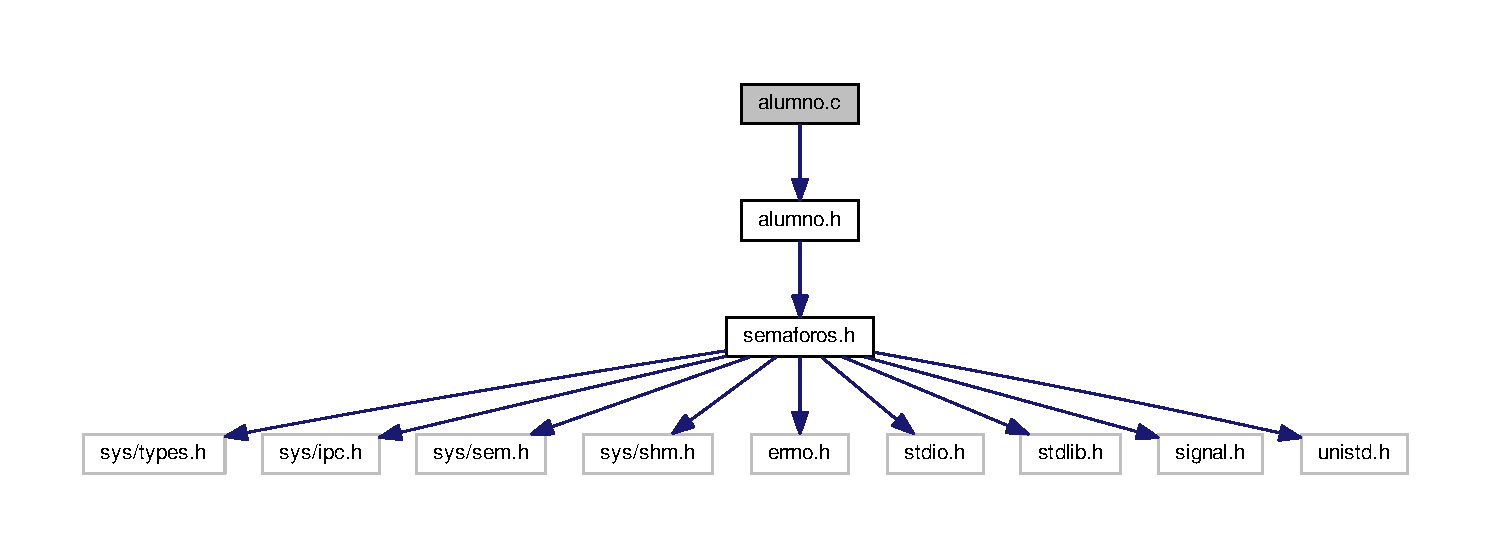
\includegraphics[width=350pt]{alumno_8c__incl}
\end{center}
\end{figure}
\subsection*{Functions}
\begin{DoxyCompactItemize}
\item 
\hypertarget{alumno_8c_afc491f44f9a3771e97dc0256075f0f52}{void \hyperlink{alumno_8c_afc491f44f9a3771e97dc0256075f0f52}{manejador\+\_\+\+S\+I\+G\+T\+E\+R\+M} (int sig)}\label{alumno_8c_afc491f44f9a3771e97dc0256075f0f52}

\begin{DoxyCompactList}\small\item\em Manejador para S\+I\+G\+T\+E\+R\+M Hace que el alumno termine. \end{DoxyCompactList}\item 
\hypertarget{alumno_8c_a26c2a6706d70bdcdd103803e84e330bd}{void \hyperlink{alumno_8c_a26c2a6706d70bdcdd103803e84e330bd}{realizar\+\_\+examen} ()}\label{alumno_8c_a26c2a6706d70bdcdd103803e84e330bd}

\begin{DoxyCompactList}\small\item\em simula realizacion el examen El alumno avisa cuando empeiza, duerme alatoriamente y avisa cuando despierta \end{DoxyCompactList}\item 
void \hyperlink{alumno_8c_a952d3a6fb2c9079f1dbf8160f53efdc3}{gestion\+\_\+alumno} (int pid, int id\+\_\+cola)
\begin{DoxyCompactList}\small\item\em Alumno Gestiona lo que realiza el proceso alumno. \end{DoxyCompactList}\end{DoxyCompactItemize}


\subsection{Detailed Description}
El alumno del proyecto de la Practica 4 S\+O\+P\+E\+R. 

\begin{DoxyAuthor}{Author}
Oscar Garcia de Lara Parreño 

Santiago Gomez Aguirre 
\end{DoxyAuthor}
\begin{DoxyVersion}{Version}
1.\+0 
\end{DoxyVersion}
\begin{DoxyDate}{Date}
29-\/04-\/2016 
\end{DoxyDate}


\subsection{Function Documentation}
\hypertarget{alumno_8c_a952d3a6fb2c9079f1dbf8160f53efdc3}{\index{alumno.\+c@{alumno.\+c}!gestion\+\_\+alumno@{gestion\+\_\+alumno}}
\index{gestion\+\_\+alumno@{gestion\+\_\+alumno}!alumno.\+c@{alumno.\+c}}
\subsubsection[{gestion\+\_\+alumno}]{\setlength{\rightskip}{0pt plus 5cm}void gestion\+\_\+alumno (
\begin{DoxyParamCaption}
\item[{int}]{pid, }
\item[{int}]{id\+\_\+cola}
\end{DoxyParamCaption}
)}}\label{alumno_8c_a952d3a6fb2c9079f1dbf8160f53efdc3}


Alumno Gestiona lo que realiza el proceso alumno. 


\begin{DoxyParams}{Parameters}
{\em pid} & pid del proceso \\
\hline
{\em id\+\_\+cola} & id de la cola de mensajes \\
\hline
\end{DoxyParams}

\hypertarget{ejercicio1_8c}{\section{ejercicio1.\+c File Reference}
\label{ejercicio1_8c}\index{ejercicio1.\+c@{ejercicio1.\+c}}
}


El ejercicio 1 de la Practica 4 S\+O\+P\+E\+R.  


{\ttfamily \#include $<$sys/types.\+h$>$}\\*
{\ttfamily \#include $<$sys/ipc.\+h$>$}\\*
{\ttfamily \#include $<$sys/msg.\+h$>$}\\*
{\ttfamily \#include $<$stdio.\+h$>$}\\*
{\ttfamily \#include $<$stdlib.\+h$>$}\\*
{\ttfamily \#include $<$string.\+h$>$}\\*
{\ttfamily \#include $<$sys/wait.\+h$>$}\\*
Include dependency graph for ejercicio1.\+c\+:
\nopagebreak
\begin{figure}[H]
\begin{center}
\leavevmode
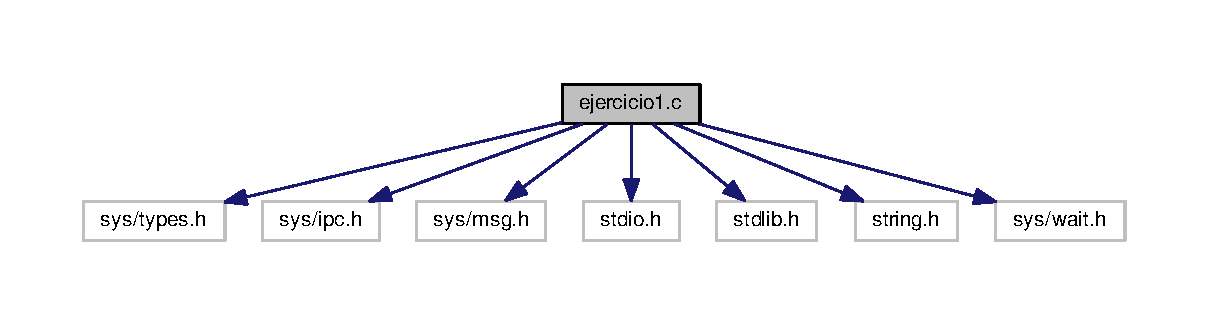
\includegraphics[width=350pt]{ejercicio1_8c__incl}
\end{center}
\end{figure}
\subsection*{Classes}
\begin{DoxyCompactItemize}
\item 
struct \hyperlink{struct__Mensaje}{\+\_\+\+Mensaje}
\begin{DoxyCompactList}\small\item\em Mensaje. \end{DoxyCompactList}\end{DoxyCompactItemize}
\subsection*{Typedefs}
\begin{DoxyCompactItemize}
\item 
typedef struct \hyperlink{struct__Mensaje}{\+\_\+\+Mensaje} \hyperlink{ejercicio1_8c_a0b62810db7104177e9427c356d59277e}{mensaje}
\begin{DoxyCompactList}\small\item\em Mensaje. \end{DoxyCompactList}\end{DoxyCompactItemize}
\subsection*{Functions}
\begin{DoxyCompactItemize}
\item 
int \hyperlink{ejercicio1_8c_abf9e6b7e6f15df4b525a2e7705ba3089}{main} (int argc, char const $\ast$argv\mbox{[}$\,$\mbox{]})
\begin{DoxyCompactList}\small\item\em Varios procesos se comunican a traves de colas de mensajes Los procesos se comunican entre si para pasar el contenido de un fichero a otro pero todos los caracteres a mayusculas. \end{DoxyCompactList}\end{DoxyCompactItemize}


\subsection{Detailed Description}
El ejercicio 1 de la Practica 4 S\+O\+P\+E\+R. 

\begin{DoxyAuthor}{Author}
Oscar Garcia de Lara Parreño 

Santiago Gomez Aguirre 
\end{DoxyAuthor}
\begin{DoxyVersion}{Version}
1.\+0 
\end{DoxyVersion}
\begin{DoxyDate}{Date}
29-\/04-\/2016 
\end{DoxyDate}


\subsection{Typedef Documentation}
\hypertarget{ejercicio1_8c_a0b62810db7104177e9427c356d59277e}{\index{ejercicio1.\+c@{ejercicio1.\+c}!mensaje@{mensaje}}
\index{mensaje@{mensaje}!ejercicio1.\+c@{ejercicio1.\+c}}
\subsubsection[{mensaje}]{\setlength{\rightskip}{0pt plus 5cm}typedef struct {\bf \+\_\+\+Mensaje} {\bf mensaje}}}\label{ejercicio1_8c_a0b62810db7104177e9427c356d59277e}


Mensaje. 

Esta estructura define un mensaje. 

\subsection{Function Documentation}
\hypertarget{ejercicio1_8c_abf9e6b7e6f15df4b525a2e7705ba3089}{\index{ejercicio1.\+c@{ejercicio1.\+c}!main@{main}}
\index{main@{main}!ejercicio1.\+c@{ejercicio1.\+c}}
\subsubsection[{main}]{\setlength{\rightskip}{0pt plus 5cm}int main (
\begin{DoxyParamCaption}
\item[{int}]{argc, }
\item[{char const $\ast$}]{argv\mbox{[}$\,$\mbox{]}}
\end{DoxyParamCaption}
)}}\label{ejercicio1_8c_abf9e6b7e6f15df4b525a2e7705ba3089}


Varios procesos se comunican a traves de colas de mensajes Los procesos se comunican entre si para pasar el contenido de un fichero a otro pero todos los caracteres a mayusculas. 

\begin{DoxyReturn}{Returns}
E\+X\+I\+T\+\_\+\+F\+A\+I\+L\+U\+R\+E en caso de error, E\+X\+I\+T\+\_\+\+S\+U\+C\+C\+E\+S\+S si funciona 
\end{DoxyReturn}

\hypertarget{gestion_8c}{\section{gestion.\+c File Reference}
\label{gestion_8c}\index{gestion.\+c@{gestion.\+c}}
}


El gestion del proyecto de la Practica 4 S\+O\+P\+E\+R.  


{\ttfamily \#include $<$string.\+h$>$}\\*
{\ttfamily \#include $<$sys/msg.\+h$>$}\\*
{\ttfamily \#include $<$sys/wait.\+h$>$}\\*
{\ttfamily \#include $<$stdio.\+h$>$}\\*
{\ttfamily \#include $<$stdlib.\+h$>$}\\*
{\ttfamily \#include \char`\"{}semaforos.\+h\char`\"{}}\\*
Include dependency graph for gestion.\+c\+:
\nopagebreak
\begin{figure}[H]
\begin{center}
\leavevmode
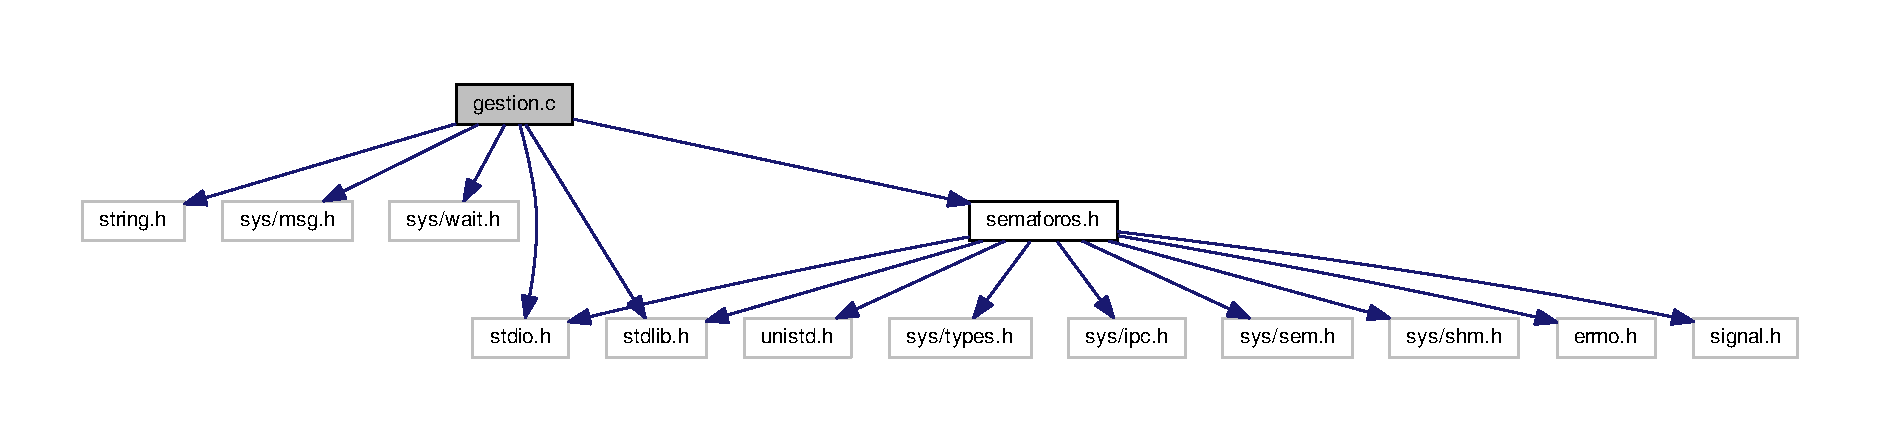
\includegraphics[width=350pt]{gestion_8c__incl}
\end{center}
\end{figure}
\subsection*{Macros}
\begin{DoxyCompactItemize}
\item 
\hypertarget{gestion_8c_a68c15c5fb7f7c6f707903e6a46ab0557}{\#define {\bfseries F\+I\+L\+E\+K\+E\+Y}~\char`\"{}/bin/cat\char`\"{}}\label{gestion_8c_a68c15c5fb7f7c6f707903e6a46ab0557}

\item 
\hypertarget{gestion_8c_a8ae9d53f33f46cfcfcb9736e6351452a}{\#define {\bfseries K\+E\+Y}~1300}\label{gestion_8c_a8ae9d53f33f46cfcfcb9736e6351452a}

\end{DoxyCompactItemize}
\subsection*{Functions}
\begin{DoxyCompactItemize}
\item 
\hypertarget{gestion_8c_a9bfeb6a95d4f270c4e435e9fec5ef1fa}{void \hyperlink{gestion_8c_a9bfeb6a95d4f270c4e435e9fec5ef1fa}{manejador\+\_\+\+S\+I\+G\+A\+L\+R\+M\+\_\+30} (int sig)}\label{gestion_8c_a9bfeb6a95d4f270c4e435e9fec5ef1fa}

\begin{DoxyCompactList}\small\item\em Manejador para la alarma de 30 segundos Lanza un comando para generar un fichero. \end{DoxyCompactList}\item 
int \hyperlink{gestion_8c_a0ddf1224851353fc92bfbff6f499fa97}{main} (int argc, char $\ast$argv\mbox{[}$\,$\mbox{]})
\begin{DoxyCompactList}\small\item\em Proceso main(\+Gestion) del simulador Se encargade pedir el numero de asientos y alumnos de la simulacion, y lanzar todos los procesos. \end{DoxyCompactList}\end{DoxyCompactItemize}


\subsection{Detailed Description}
El gestion del proyecto de la Practica 4 S\+O\+P\+E\+R. 

\begin{DoxyAuthor}{Author}
Oscar Garcia de Lara Parreño 

Santiago Gomez Aguirre 
\end{DoxyAuthor}
\begin{DoxyVersion}{Version}
1.\+0 
\end{DoxyVersion}
\begin{DoxyDate}{Date}
29-\/04-\/2016 
\end{DoxyDate}


\subsection{Function Documentation}
\hypertarget{gestion_8c_a0ddf1224851353fc92bfbff6f499fa97}{\index{gestion.\+c@{gestion.\+c}!main@{main}}
\index{main@{main}!gestion.\+c@{gestion.\+c}}
\subsubsection[{main}]{\setlength{\rightskip}{0pt plus 5cm}int main (
\begin{DoxyParamCaption}
\item[{int}]{argc, }
\item[{char $\ast$}]{argv\mbox{[}$\,$\mbox{]}}
\end{DoxyParamCaption}
)}}\label{gestion_8c_a0ddf1224851353fc92bfbff6f499fa97}


Proceso main(\+Gestion) del simulador Se encargade pedir el numero de asientos y alumnos de la simulacion, y lanzar todos los procesos. 

\begin{DoxyReturn}{Returns}
E\+X\+I\+T\+\_\+\+F\+A\+I\+L\+U\+R\+E en caso de error, E\+X\+I\+T\+\_\+\+S\+U\+C\+C\+E\+S\+S si funciona 
\end{DoxyReturn}

\hypertarget{profesor_8c}{\section{profesor.\+c File Reference}
\label{profesor_8c}\index{profesor.\+c@{profesor.\+c}}
}


El profesor del proyecto de la Practica 4 S\+O\+P\+E\+R.  


{\ttfamily \#include \char`\"{}profesor.\+h\char`\"{}}\\*
Include dependency graph for profesor.\+c\+:
\nopagebreak
\begin{figure}[H]
\begin{center}
\leavevmode
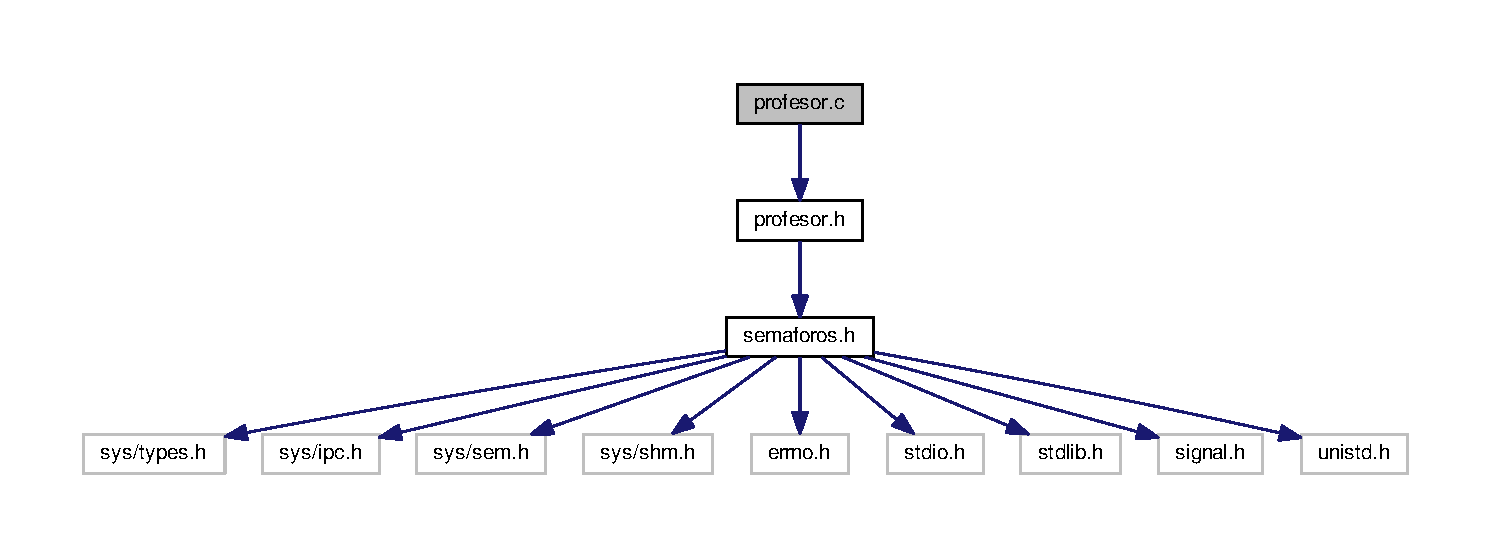
\includegraphics[width=350pt]{profesor_8c__incl}
\end{center}
\end{figure}
\subsection*{Functions}
\begin{DoxyCompactItemize}
\item 
\hypertarget{profesor_8c_a4f970554c0f5991016f3caeb73fe7578}{void \hyperlink{profesor_8c_a4f970554c0f5991016f3caeb73fe7578}{manejador\+\_\+\+S\+I\+G\+A\+L\+R\+M\+\_\+5} (int sig)}\label{profesor_8c_a4f970554c0f5991016f3caeb73fe7578}

\begin{DoxyCompactList}\small\item\em Manejador para la alarma de 5 minutos Obliga a terminar el examen a los alumnos que lo estan realizando. \end{DoxyCompactList}\item 
void \hyperlink{profesor_8c_ab06fad87d99b4e5ad78c40afa4829521}{gestion\+\_\+profesor} (int pid, \hyperlink{structAula}{Aula} $\ast$aula, int num\+\_\+aula, int id\+\_\+cola, int id\+Mutex)
\begin{DoxyCompactList}\small\item\em Profesor Gestiona lo que realiza el proceso profesor. \end{DoxyCompactList}\item 
void \hyperlink{profesor_8c_a9bf602e55db8fdc42f00d45bd8bf3554}{gestion\+\_\+profesor\+\_\+examen} (int pid, \hyperlink{structAula}{Aula} $\ast$aula, int num\+\_\+aula, int id\+\_\+cola, int id\+Mutex)
\begin{DoxyCompactList}\small\item\em Profesor\+\_\+examen Gestiona lo que realiza el proceso profesor\+\_\+examen. \end{DoxyCompactList}\item 
int \hyperlink{profesor_8c_a6319aea0759e646e7b3e97b5b646ffe6}{comprobacion\+\_\+aula} (\hyperlink{structAula}{Aula} $\ast$aula)
\begin{DoxyCompactList}\small\item\em Comprobacion\+\_\+aula Comprueba que el aula este disponible. \end{DoxyCompactList}\end{DoxyCompactItemize}
\subsection*{Variables}
\begin{DoxyCompactItemize}
\item 
\hypertarget{profesor_8c_a172d23db2d6c23b1daea27d16c8316e6}{\hyperlink{structAula}{Aula} $\ast$ {\bfseries aulag}}\label{profesor_8c_a172d23db2d6c23b1daea27d16c8316e6}

\item 
\hypertarget{profesor_8c_adf611b6d315dbf8b63641ecedca82867}{int {\bfseries num\+\_\+aulag}}\label{profesor_8c_adf611b6d315dbf8b63641ecedca82867}

\item 
\hypertarget{profesor_8c_aeeb80ff72b5505d0644b2b9972e556bc}{int {\bfseries idmutexg}}\label{profesor_8c_aeeb80ff72b5505d0644b2b9972e556bc}

\end{DoxyCompactItemize}


\subsection{Detailed Description}
El profesor del proyecto de la Practica 4 S\+O\+P\+E\+R. 

\begin{DoxyAuthor}{Author}
Oscar Garcia de Lara Parreño 

Santiago Gomez Aguirre 
\end{DoxyAuthor}
\begin{DoxyVersion}{Version}
1.\+0 
\end{DoxyVersion}
\begin{DoxyDate}{Date}
29-\/04-\/2016 
\end{DoxyDate}


\subsection{Function Documentation}
\hypertarget{profesor_8c_a6319aea0759e646e7b3e97b5b646ffe6}{\index{profesor.\+c@{profesor.\+c}!comprobacion\+\_\+aula@{comprobacion\+\_\+aula}}
\index{comprobacion\+\_\+aula@{comprobacion\+\_\+aula}!profesor.\+c@{profesor.\+c}}
\subsubsection[{comprobacion\+\_\+aula}]{\setlength{\rightskip}{0pt plus 5cm}int comprobacion\+\_\+aula (
\begin{DoxyParamCaption}
\item[{{\bf Aula} $\ast$}]{aula}
\end{DoxyParamCaption}
)}}\label{profesor_8c_a6319aea0759e646e7b3e97b5b646ffe6}


Comprobacion\+\_\+aula Comprueba que el aula este disponible. 


\begin{DoxyParams}{Parameters}
{\em $\ast$aula} & array de aulas \\
\hline
\end{DoxyParams}
\hypertarget{profesor_8c_ab06fad87d99b4e5ad78c40afa4829521}{\index{profesor.\+c@{profesor.\+c}!gestion\+\_\+profesor@{gestion\+\_\+profesor}}
\index{gestion\+\_\+profesor@{gestion\+\_\+profesor}!profesor.\+c@{profesor.\+c}}
\subsubsection[{gestion\+\_\+profesor}]{\setlength{\rightskip}{0pt plus 5cm}void gestion\+\_\+profesor (
\begin{DoxyParamCaption}
\item[{int}]{pid, }
\item[{{\bf Aula} $\ast$}]{aula, }
\item[{int}]{num\+\_\+aula, }
\item[{int}]{id\+\_\+cola, }
\item[{int}]{id\+Mutex}
\end{DoxyParamCaption}
)}}\label{profesor_8c_ab06fad87d99b4e5ad78c40afa4829521}


Profesor Gestiona lo que realiza el proceso profesor. 


\begin{DoxyParams}{Parameters}
{\em pid} & pid del proceso \\
\hline
{\em $\ast$aula} & array de aulas \\
\hline
{\em num\+\_\+aula} & numero del aula en el que esta asignado (0 o 1) \\
\hline
{\em id\+\_\+cola} & id de la cola de mensajes \\
\hline
{\em id\+Mutex} & id del semafaro Mutex \\
\hline
\end{DoxyParams}
\hypertarget{profesor_8c_a9bf602e55db8fdc42f00d45bd8bf3554}{\index{profesor.\+c@{profesor.\+c}!gestion\+\_\+profesor\+\_\+examen@{gestion\+\_\+profesor\+\_\+examen}}
\index{gestion\+\_\+profesor\+\_\+examen@{gestion\+\_\+profesor\+\_\+examen}!profesor.\+c@{profesor.\+c}}
\subsubsection[{gestion\+\_\+profesor\+\_\+examen}]{\setlength{\rightskip}{0pt plus 5cm}void gestion\+\_\+profesor\+\_\+examen (
\begin{DoxyParamCaption}
\item[{int}]{pid, }
\item[{{\bf Aula} $\ast$}]{aula, }
\item[{int}]{num\+\_\+aula, }
\item[{int}]{id\+\_\+cola, }
\item[{int}]{id\+Mutex}
\end{DoxyParamCaption}
)}}\label{profesor_8c_a9bf602e55db8fdc42f00d45bd8bf3554}


Profesor\+\_\+examen Gestiona lo que realiza el proceso profesor\+\_\+examen. 


\begin{DoxyParams}{Parameters}
{\em pid} & pid del proceso \\
\hline
{\em $\ast$aula} & array de aulas \\
\hline
{\em num\+\_\+aula} & numero del aula en el que esta asignado (0 o 1) \\
\hline
{\em id\+\_\+cola} & id de la cola de mensajes \\
\hline
{\em id\+Mutex} & id del semafaro Mutex \\
\hline
\end{DoxyParams}

\hypertarget{semaforos_8h}{\section{semaforos.\+h File Reference}
\label{semaforos_8h}\index{semaforos.\+h@{semaforos.\+h}}
}


\hyperlink{semaforos_8h}{semaforos.\+h}  


{\ttfamily \#include $<$sys/types.\+h$>$}\\*
{\ttfamily \#include $<$sys/ipc.\+h$>$}\\*
{\ttfamily \#include $<$sys/sem.\+h$>$}\\*
{\ttfamily \#include $<$sys/shm.\+h$>$}\\*
{\ttfamily \#include $<$errno.\+h$>$}\\*
{\ttfamily \#include $<$stdio.\+h$>$}\\*
{\ttfamily \#include $<$stdlib.\+h$>$}\\*
{\ttfamily \#include $<$signal.\+h$>$}\\*
{\ttfamily \#include $<$unistd.\+h$>$}\\*
Include dependency graph for semaforos.\+h\+:
\nopagebreak
\begin{figure}[H]
\begin{center}
\leavevmode
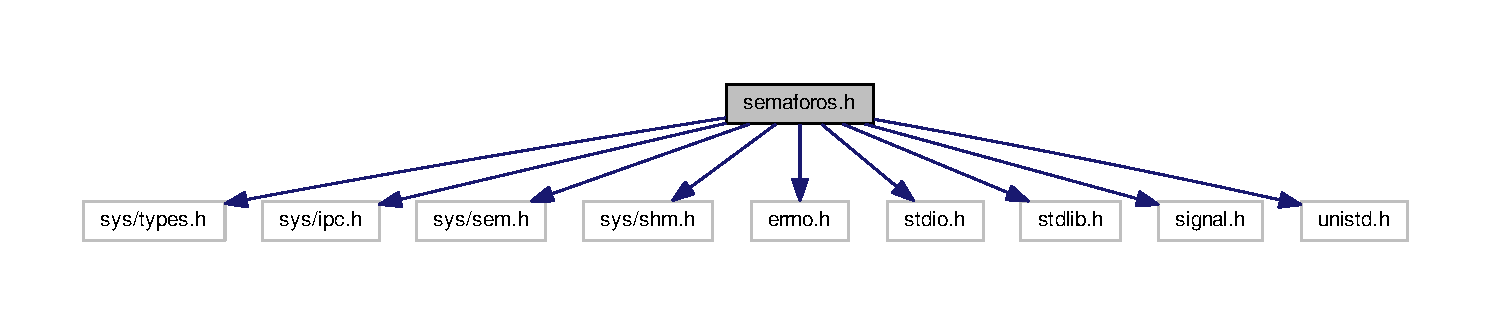
\includegraphics[width=350pt]{semaforos_8h__incl}
\end{center}
\end{figure}
This graph shows which files directly or indirectly include this file\+:
\nopagebreak
\begin{figure}[H]
\begin{center}
\leavevmode
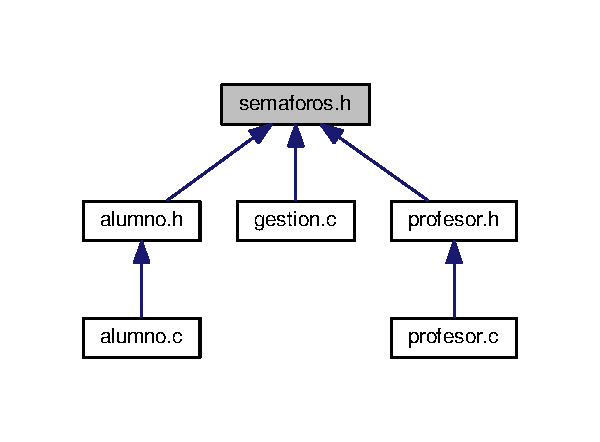
\includegraphics[width=288pt]{semaforos_8h__dep__incl}
\end{center}
\end{figure}
\subsection*{Classes}
\begin{DoxyCompactItemize}
\item 
struct \hyperlink{struct__Mensaje}{\+\_\+\+Mensaje}
\begin{DoxyCompactList}\small\item\em Mensaje. \end{DoxyCompactList}\item 
struct \hyperlink{structAula}{Aula}
\begin{DoxyCompactList}\small\item\em \hyperlink{structAula}{Aula}. \end{DoxyCompactList}\end{DoxyCompactItemize}
\subsection*{Typedefs}
\begin{DoxyCompactItemize}
\item 
typedef struct \hyperlink{struct__Mensaje}{\+\_\+\+Mensaje} \hyperlink{semaforos_8h_a0b62810db7104177e9427c356d59277e}{mensaje}
\begin{DoxyCompactList}\small\item\em Mensaje. \end{DoxyCompactList}\end{DoxyCompactItemize}
\subsection*{Enumerations}
\begin{DoxyCompactItemize}
\item 
\hypertarget{semaforos_8h_a32c27cc471df37f4fc818d65de0a56c4}{enum {\bfseries S\+T\+A\+T\+U\+S} \{ {\bfseries O\+K} =0, 
{\bfseries E\+R\+R\+O\+R} =-\/1
 \}}\label{semaforos_8h_a32c27cc471df37f4fc818d65de0a56c4}

\end{DoxyCompactItemize}
\subsection*{Functions}
\begin{DoxyCompactItemize}
\item 
\hypertarget{semaforos_8h_a4af104b0ed37e6ae0289a1059bc6e990}{int {\bfseries Inicializar\+\_\+\+Semaforo} (int semid, unsigned short $\ast$array)}\label{semaforos_8h_a4af104b0ed37e6ae0289a1059bc6e990}

\item 
\hypertarget{semaforos_8h_a731339337960a681efa435a10f12c312}{int {\bfseries Borrar\+\_\+\+Semaforo} (int semid)}\label{semaforos_8h_a731339337960a681efa435a10f12c312}

\item 
\hypertarget{semaforos_8h_a16b16dd895b5f4cbe48f1ac8977e8b35}{int {\bfseries Crear\+\_\+\+Semaforo} (key\+\_\+t key, int size, int $\ast$semid)}\label{semaforos_8h_a16b16dd895b5f4cbe48f1ac8977e8b35}

\item 
\hypertarget{semaforos_8h_a883244cd3b83c42cda23687da1b63369}{int {\bfseries Down\+\_\+\+Semaforo} (int id, int num\+\_\+sem, int undo)}\label{semaforos_8h_a883244cd3b83c42cda23687da1b63369}

\item 
\hypertarget{semaforos_8h_ab375ebfc38acbdced46e062a689d5fad}{int {\bfseries Down\+Multiple\+\_\+\+Semaforo} (int id, int size, int undo, int $\ast$active)}\label{semaforos_8h_ab375ebfc38acbdced46e062a689d5fad}

\item 
\hypertarget{semaforos_8h_a2d5e735aecee4f493898b3d4ebab1a10}{int {\bfseries Up\+\_\+\+Semaforo} (int id, int num\+\_\+sem, int undo)}\label{semaforos_8h_a2d5e735aecee4f493898b3d4ebab1a10}

\item 
\hypertarget{semaforos_8h_a943759695f018d64a94b8a2c49308092}{int {\bfseries Up\+Multiple\+\_\+\+Semaforo} (int id, int size, int undo, int $\ast$active)}\label{semaforos_8h_a943759695f018d64a94b8a2c49308092}

\end{DoxyCompactItemize}


\subsection{Detailed Description}
\hyperlink{semaforos_8h}{semaforos.\+h} 

\begin{DoxyAuthor}{Author}
Oscar Garcia de Lara Parreño 

Santiago Gomez Aguirre 
\end{DoxyAuthor}
\begin{DoxyVersion}{Version}
1.\+0 
\end{DoxyVersion}
\begin{DoxyDate}{Date}
29-\/03¡4-\/2016 
\end{DoxyDate}


\subsection{Typedef Documentation}
\hypertarget{semaforos_8h_a0b62810db7104177e9427c356d59277e}{\index{semaforos.\+h@{semaforos.\+h}!mensaje@{mensaje}}
\index{mensaje@{mensaje}!semaforos.\+h@{semaforos.\+h}}
\subsubsection[{mensaje}]{\setlength{\rightskip}{0pt plus 5cm}typedef struct {\bf \+\_\+\+Mensaje} {\bf mensaje}}}\label{semaforos_8h_a0b62810db7104177e9427c356d59277e}


Mensaje. 

Esta estructura define un mensaje. 
%--- End generated contents ---

% Index
\newpage
\phantomsection
\addcontentsline{toc}{chapter}{Index}
\printindex

\end{document}
